\scanpage{36}
\unsure{Supposons} les $\beta_i\inserted{=\alpha_i+2}$ inv.
\[
\begin{array}{rcl}
\text{forme sur }\unsure{\mathcal L}(a_{i-1},a_i,a_{i+1})\text{ lisse}
&\Longleftrightarrow&\alpha_{i-1}+\alpha_i\quad\text{inv.}\\
\text{forme sur }\unsure{\mathcal L}(a_{i-1},a_i)\text{ lisse}
&\Longleftrightarrow&2-\alpha_{i-1}\quad\text{inv.}\\
\longrightarrow\quad\unsure{\mathcal L}(a_i,a_{i+1})\text{ lisse}
&\Longleftrightarrow&2-\alpha_i\quad\text{inv.}
\end{array}
\]
\deleted{$\unsure{\alpha_i}$}
\figure{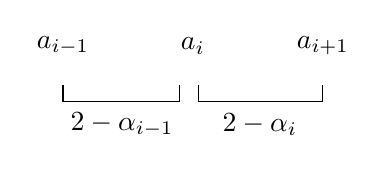
\begin{tikzpicture}[x=1cm,y=1cm]
\node at (0,0.45) {$a_{i-1}$}; \node at (1.65,0.45) {$a_i$}; \node at (3.3,0.45) {$a_{i+1}$};
\draw (0,-0.05)--(0,-0.25)--(1.48,-0.25)--(1.48,-0.05);
\draw (1.72,-0.05)--(1.72,-0.25)--(3.3,-0.25)--(3.3,-0.05);
\node at (.75,-.55) {$2-\unsure{\alpha_{i-1}}$}; \node at (2.5,-.55) {$2-\alpha_i$};
\end{tikzpicture}}
$\alpha_i\ne2$. \unsure{pas} de val. propres $1$
\[
\alpha_{\unsure{i-1}}\ne2.
\]
\deleted{\unsure{Ret.}} Si
\margin{Sur $1\le i\unsure{\leq|<}n-1$}
\diagram{\begin{tikzcd}[ampersand replacement=\&,column sep=large,row sep=small]
\& |[draw,rounded corners]| \text{donc car. }\ne2!\\
\left.\begin{array}{l}
\beta_0,\ldots,\beta_{n-1}\quad\text{inv.}\\
2(\alpha_{i-1}+\alpha_i)\quad\text{inv.}\\
\alpha_{i-1}-2,\ \alpha_i-2\quad\text{inv.}
\end{array}\right\}\arrow[ur] \&
\end{tikzcd}}
alors $\tau_i$ se reconstruit à partir des
$\underset{\substack{\Vert\\\tau_{i-1}\tau_i}}{\rho_{i-1}},\
\underset{\substack{\Vert\\\tau_i\tau_{i+1}}}{\rho_i}$,
donc aussi
\[
\tau_{i-1}=\rho_{i-1}\tau_i,\qquad
\tau_{i+1}=\tau_i\rho_i.
\]
\margin{\uline{dans $V,f$}\quad $C=\mathbb P(V)\unsure{\setminus}Q$\quad $(n\ge2)$}
$\tau_i=$ \deleted{\unsure{sym.}} réflexion associée à la \uline{direction}
\[
\begin{aligned}
\left(
\underbrace{V^{\rho_{i-1}}}_{\substack{\deleted{\unsure{\subset}}\Vert\\\{a_{i-1},a_i\}^{\perp}}}
+
\underbrace{V^{\rho_i}}_{\substack{\Vert\\\{a_i,a_{i+1}\}^{\perp}}}
\right)^\perp
&=\{a_{i-1},a_i\}^{\perp\perp}\cap\{a_i,a_{i+1}\}^{\perp\perp}\\
&=\unsure{\mathcal L}(a_{i-1},a_i)\cap\unsure{\mathcal L}(a_i,a_{i+1}).
\end{aligned}
\]
\[
\alpha_i=\frac{(a_i,a_{i+1})^2}{f(a_i)f(a_{i+1})}
=4\cos^2\theta_i\cdot\deleted{\unsure{2\cos2}}.
\]
\[
\beta_i=\alpha_i+2
=2\bigl(\underbrace{2\cos^2\theta_i+1}_{\deleted{\unsure{2}}\cos2\theta_i}\bigr)
=4\cos2\theta_i.
\]
\mspage{35}

